\documentclass[a4paper,12pt]{article}
\usepackage[utf8]{inputenc}
\usepackage{geometry}
\usepackage{array}
\usepackage{hyperref}
\usepackage{graphicx}

\newcommand\blfootnote[1]{%
  \begingroup
  \renewcommand\thefootnote{}\footnotetext{#1}%
  \addtocounter{footnote}{-1}%
  \endgroup
}

% Set margins
\geometry{top=1in, bottom=1in, left=1in, right=1in}

\begin{document}

% --- Title ---
\begin{center}
    \textbf{\Large DS3020}
    
    \vspace{0.5cm}
    
    \textbf{\Large Mid Term Project Report}
\end{center}
\vspace{0.5cm}

% --- Header Details ---
\noindent
\textbf{{Project Title}: Campus Payment system} \hfill \textbf{Date:} \today

\vspace{0.5cm}

\hline

\vspace{0.5cm}

\section*{\underline{Introduction}}
Within a campus, the typical methods of carrying out payments to vendors are cash or UPI. Some inherent limitations of these systems: cash transactions are frequently delayed by a lack of loose change, while UPI is susceptible to external banking server downtime and network failures. This project aims to complement existing systems using a local and centralized system while also providing additional utilities like spending history and spending limits.\\

Here, we design a unified campus payment system where students can maintain their virtual bank accounts in SAC and make payments conveniently without carrying the concerns about money. The students are supposed to deposit an additional amount along with their semester fee payments which is stored in these SAC accounts. They can both recharge this account when required and use the available balance to pay for bills at campus amenities. \\
The student's balance is updated immediately when a bill is generated at a shop but the vendor is credited only after the admin approves a batch of bills as a settlement.\\

The system aims to provide several additional features to improve convenience and transparency. Students can view their complete transaction history and monitor their spending patterns. They can set spending limits for stipulated time periods. Administrators are responsible to ensure the integrity of the system by approving settlements and monitoring transactions. Moreover, there will be provisions for students to check the availability of products in any store and compare the prices for the same product at different vendors to make her life easier.

\blfootnote{All files related to this project are added \href{https://github.com/madhavpnair/Campus-Payment-system}{here}}

\newpage

\section*{\underline{ER Model}}

\subsection*{\underline{Entities}}

\begin{figure}[h!] % [h!] forces the image to appear "here"
    \centering
    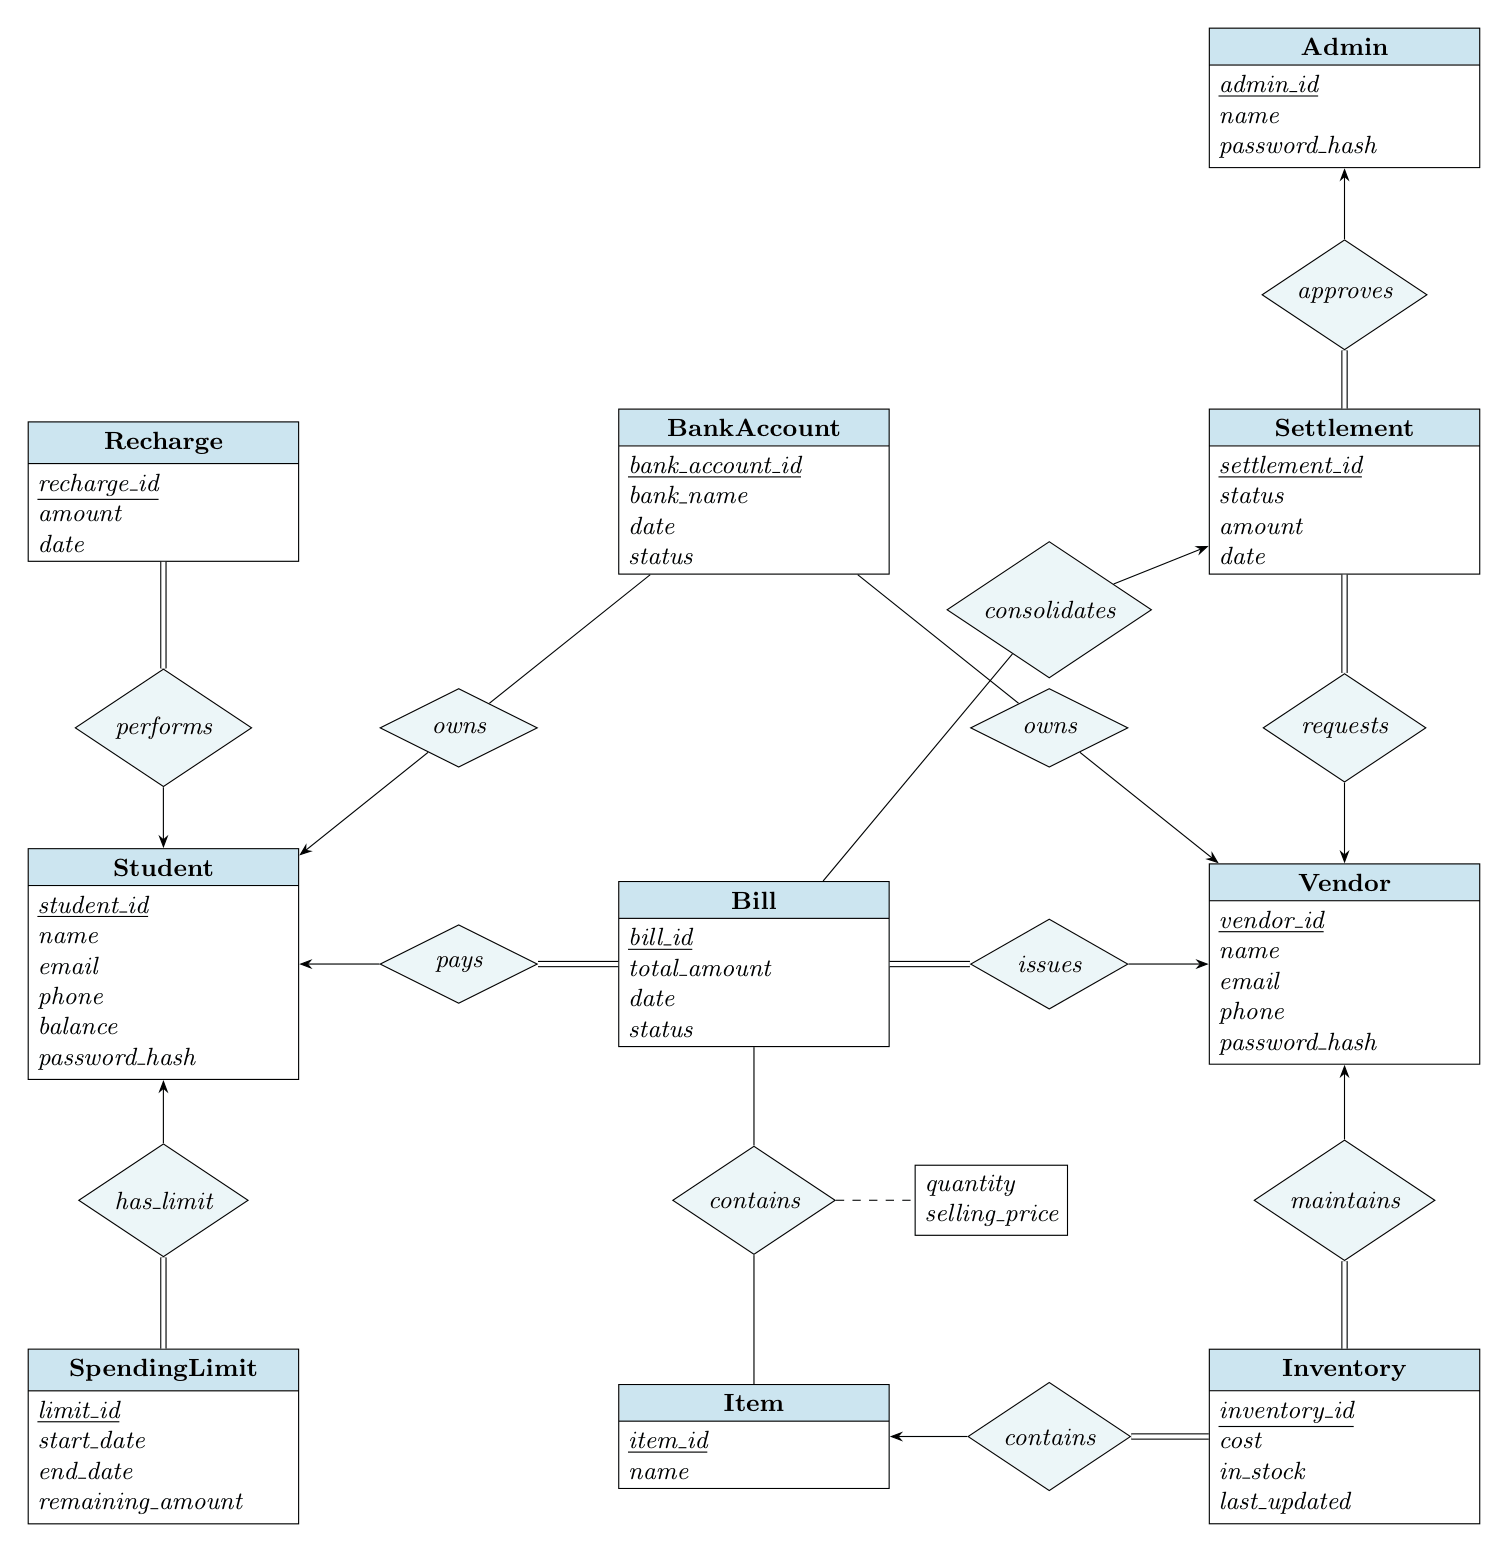
\includegraphics[width=0.8\textwidth]{assets/er.png} 
    \caption{ER Diagram}
    \label{fig:er_diagram}
\end{figure}


The details of the entities and their attributes used in the model are given below:

\begin{enumerate}
    \item \textbf{Student}
    \begin{itemize}
        \item \textbf{Primary key}: \textit{student\_id}
        \item Attributes include \textit{student\_id}, \textit{name}, \textit{email}, \textit{phone}, \textit{balance} and \textit{password\_hash}.
        \item \textit{balance} denotes the remaining amount the student can use for carrying out purchases. This can be increased by performing a recharge.
        \item Participates in 4 relationships - \textit{performs} (with \textbf{Recharge}), \textit{owns} (with \textbf{BankAccount}), \textit{pays} (with \textbf{Bill}), \textit{has\_limit} (with \textbf{SpendingLimit})
    \end{itemize}
    
    \item \textbf{Vendor}
    \begin{itemize}
        \item \textbf{Primary key}: \textit{vendor\_id}
        \item Attributes include \textit{vendor\_id}, \textit{name}, \textit{email}, \textit{phone} and \textit{password\_hash}.
        \item Participates in 4 relationships - \textit{request} (with \textbf{Settlement}), \textit{owns} (with \textbf{BankAccount}), \textit{maintains} (with \textbf{Inventory}), \textit{issues} (with \textbf{Bill}).
    \end{itemize}
    
    \item \textbf{Admin}
    \begin{itemize}
        \item \textbf{Primary key}: \textit{admin\_id}
        \item Attributes include \textit{admin\_id}, \textit{name}, \textit{email},  and \textit{password\_hash}.
        \item Participates in 1 relationship - \textit{approves} (with \textbf{Settlement}).
    \end{itemize}
    
    \item \textbf{Inventory}
    \begin{itemize}
        \item \textbf{Primary key}: \textit{inventory\_id}
        \item Attributes include \textit{inventory\_id}, \textit{cost}, \textit{in\_stock}, \textit{last\_updates}.
        \item \textit{in\_stock} is a boolean value which indicates whether an item is in stock with a particular vendor currently.
        \item Participates in 2 relationships - \textit{contains} (with \textbf{Item}) and \textit{maintains} (with \textbf{Vendor}).
    \end{itemize}
    
    \item \textbf{Bill}
    \begin{itemize}
        \item \textbf{Primary key}: \textit{bill\_id}
        \item Attributes include \textit{bill\_id}, \textit{total\_amount}, \textit{date} and \textit{status}.
        \item \textit{status} indicates whether a transaction related to a bill was completed or not.
        \item Participates in 4 relationships - \textit{consolidates} (with \textbf{Settlement}), \textit{issues} (with \textbf{Vendor}), \textit{pays} (with \textbf{Student}) and \textit{contains} (with \textbf{Item}).
    \end{itemize}
    
    \item \textbf{Item}
    \begin{itemize}
        \item \textbf{Primary key}: \textit{item\_id}
        \item Attributes include \textit{item\_id}, \textit{name}.
        \item Participates in 2 relationships - \textit{contains} (with \textbf{Bill}) and  \textit{contains} (with \textbf{Inventory}).
    \end{itemize}
    
    \item \textbf{Settlement}
    \begin{itemize}
        \item \textbf{Primary key}: \textit{settlement\_id}
        \item Attributes include \textit{settlement\_id}, \textit{status}, \textit{amount} and \textit{date}.
        \item Participates in 3 relationships - \textit{approves} (with \textbf{Admin}),  \textit{consolidates} (with \textbf{Bill}), \textit{requests} (with \textbf{Vendor}).
    \end{itemize}
    
    \item \textbf{BankAccount}
    \begin{itemize}
        \item \textbf{Primary key}: \textit{bank\_account\_id}
        \item Attributes include \textit{bank\_account\_id}, \textit{bank\_name}, \textit{account\_no}, \textit{ifsc\_code}.
        \item Participates in 2 relationships - \textit{owns} (with \textbf{Vendor}), \textit{owns} (with \textbf{Student}).
    \end{itemize}
    
    \item \textbf{Recharge}
    \begin{itemize}
        \item \textbf{Primary key}: \textit{recharge\_id}
        \item Attributes include \textit{recharge\_id}, \textit{amount}, \textit{date}.
        \item Participates in 1 relationship - \textit{performs} (with \textbf{Student})
    \end{itemize}
    
    \item \textbf{SpendingLimit}
    \begin{itemize}
        \item \textbf{Primary key}: \textit{limit\_id}
        \item Attributes include \textit{limit\_id}, \textit{start\_date}, \textit{end\_date}, \textit{remaining\_amount}.
        \item Participates in 1 relationship - \textit{has\_limit} (with \textbf{Student}).
    \end{itemize}
    
\end{enumerate}

\subsection*{\underline{Relationships}}

\begin{enumerate}
    \item \textit{owns} (\textbf{Student} - \textbf{BankAccount})
    \begin{itemize}
        \item \textbf{Cardinality} - 1:N 
        \item \textbf{Participation} - Total participation from \textbf{BankAccount}
    \end{itemize}

    \item \textit{owns} (\textbf{Vendor} - \textbf{BankAccount})
    \begin{itemize}
        \item \textbf{Cardinality} - 1:N
        \item \textbf{Participation} - Total participation from \textbf{BankAccount}
    \end{itemize}

    \item \textit{performs} (\textbf{Student} - \textbf{Recharge})
    \begin{itemize}
        \item \textbf{Cardinality} - 1:N
        \item \textbf{Participation} - Total participation from \textbf{Recharge}
    \end{itemize}

    \item \textit{pays} (\textbf{Student} - \textbf{Bill})
    \begin{itemize}
        \item \textbf{Cardinality} - 1:N
        \item \textbf{Participation} -  Total participation from \textbf{Bill}
    \end{itemize}

    \item \textit{has\_limit} (\textbf{Student} - \textbf{SpendingLimit})
    \begin{itemize}
        \item \textbf{Cardinality} - 1:N
        \item \textbf{Participation} - Total participation from \textbf{BankAccount}
    \end{itemize}

    \item \textit{requests} (\textbf{Vendor} - \textbf{Settlement})
    \begin{itemize}
        \item \textbf{Cardinality} - 1:N
        \item \textbf{Participation} -  Total participation from \textbf{Settlement}
    \end{itemize}

    \item \textit{issues} (\textbf{Vendor} - \textbf{Bill})
    \begin{itemize}
        \item \textbf{Cardinality} - 1:N
        \item \textbf{Participation} - Total participation from \textbf{Bill}
    \end{itemize}

    \item \textit{maintains} (\textbf{Vendor} - \textbf{Inventory})
    \begin{itemize}
        \item \textbf{Cardinality} - 1:N
        \item \textbf{Participation} - Total participation from \textbf{Inventory}
    \end{itemize}

    \item \textit{contains} (\textbf{Bill} - \textbf{Item})
    \begin{itemize}
        \item \textbf{Cardinality} - M:N
        \item \textbf{Participation} - Total Participation from \textbf{Bill}
        \item It is a many to many relationship with \textbf{descriptive attributes} \textit{quantity}
        and \textit{selling\_price}
    \end{itemize}

    \item \textit{approves} (\textbf{Admin} - \textbf{Settlement})
    \begin{itemize}
        \item \textbf{Cardinality} - 1:N
        \item \textbf{Participation} - Total Participation from \textbf{Settlement}
    \end{itemize}

    \item \textit{consolidates} (\textbf{Settlement} - \textbf{Bill})
    \begin{itemize}
        \item \textbf{Cardinality} - 1:N
        \item \textbf{Participation} - Total Participation from \textbf{Settlement}
    \end{itemize}

    \item \textit{contains} (\textbf{Item} - \textbf{Inventory})
    \begin{itemize}
        \item \textbf{Cardinality} - 1:N
        \item \textbf{Participation} - Total Participation from \textbf{Inventory}
    \end{itemize}
\end{enumerate}

\section*{\underline{Relational Model}}

\begin{figure}[h!] % [h!] forces the image to appear "here"
    \centering
    \includegraphics[width=0.8\textwidth]{assets/relational_diagram_final.jpg} 
    \caption{ER Diagram}
    \label{fig:relational_schema}
\end{figure}
\noindent
Figure 2 shows the relational model corresponding to the proposed ER Model. \\

\noindent
All the strong entities from the ER Model are directly converted to relations. 
Their relationships are captured by adding appropriate foreign keys to appropriate sides based on cardinality constraints, which will be further explained in the general constraints section.\\\\
\noindent
Apart from these, three relations have been created for specific reasons.
\begin{itemize}
    \item The \textbf{BillItem} table breaks down the many-to-many relationship between the \textbf{Bill} and \textbf{Item} tables. 
    \item Students use SAC accounts for transactions while vendors receive money through their actual bank accounts. 
In order to account for such a distinction and to simplify the related queries, we create two tables named \textbf{StudentAccount} and \textbf{VendorAccount}.
\item The same could be realized by adding both \textit{vendor\_id} and \textit{student\_id} as foreign keys to the \textbf{BankAccount} table but its every row would have either \textit{student\_id} or \textit{vendor\_id} as NULL value which is not recommended.
\end{itemize}

\noindent
The \textbf{Bill} table references the \textit{settlement\_id} from \textbf{Settlement} table. This \textbf{FK} is \textbf{NULLABLE} and gets a valid value only once the particular bill gets settled

\section*{\underline{Functional Dependencies}}

\subsection*{1. Primary Key Dependencies}
In strong entities, the primary key uniquely identifies every other attribute in the table. These are non-trivial functional dependencies where the determinant is a candidate key
\newline
\item \textbf{Student Entity:}  \text{student\_id} \rightarrow \{\text{name, email, phone, balance, password\_hash}\} 
\item \textbf{Vendor Entity:}  \text{vendor\_id} \rightarrow \{\text{name, email, phone, password\_hash}\} 
\item \textbf{Admin Entity:} \text{admin\_id} \rightarrow \{\text{name, password\_hash}\} 
\item \textbf{Item Entity:} \text{item\_id} \rightarrow \{\text{name}\} 
\item \textbf{BankAccount Entity:} \text{bank\_account\_id} \rightarrow \{\text{bank\_name, date, status}\} 
\item \textbf{Recharge Entity:} \text{recharge\_id} \rightarrow \{\text{amount, date, student\_id}\} 
\item \textbf{SpendingLimit Entity:} \text{limit\_id} \rightarrow \{\text{start\_date, end\_date, remaining\_amount, student\_id}\} 

\subsection*{2. Associative Entity Dependencies}
Several entities and relationships resolve complex interactions (like M:N relationships) or act as bridging tables.
\newline
\item \textbf{Inventory Entity:} Acts as the bridge between a Vendor and an Item.
\[ \text{inventory\_id} \rightarrow \{\text{cost, in\_stock, last\_updated, vendor\_id, item\_id}\} \]
\item \textbf{Bill Entity:} Consolidates the transaction as the ``Header'' of a receipt.
\[ \text{bill\_id} \rightarrow \{\text{total\_amount, date, status, student\_id, vendor\_id}\} \]
\item \textbf{Settlement Entity:} Determines the clearing of funds.
\[ \text{settlement\_id} \rightarrow \{\text{status, amount, date, vendor\_id, admin\_id}\} \]

\subsection*{3. Composite Key Dependencies}
For entities that resolve many-to-many relationships, functional dependencies rely on a \newline  composite determinant (a combination of foreign keys acting as the primary key)
\newline
\item \textbf{Bill\_Items:} Neither the bill\_id nor the item\_id can alone determine the quantity or the \newline selling\_price.
    \[ \{\text{bill\_id, item\_id}\} \rightarrow \{\text{quantity, selling\_price}\} \]
    
\newpage
\section*{\underline{Tables and General Constraints}}

\begin{enumerate}
    \item \textbf{Admin}
    \begin{center}
        \includegraphics[width=1\textwidth]{assets/tables/admin.png}
    \end{center}
    \textbf{Primary Key Constraint}:
    \begin{itemize}
        \item admin\_pkey (student\_id)
    \end{itemize}

\newpage
    \item \textbf{Bank\_Account}
    \begin{center}
        \includegraphics[width=1\textwidth]{assets/tables/bank_account.png}
    \end{center}
    \textbf{Primary Key Constraint}:
    \begin{itemize}
        \item bank\_account\_pkey (bankaccount\_id)
    \end{itemize}
\newpage
    \item \textbf{Bill}
    \begin{center}
        \includegraphics[width=1\textwidth]{assets/tables/bill.png}
    \end{center}
    \textbf{Primary Key Constraint}:
    \begin{itemize}
        \item bill\_pkey (bill\_id)
    \end{itemize}

    \textbf{Foreign Key Constraints}:
    \begin{itemize}
        \item fk\_settlement (settlement\_id $\rightarrow$ settlement.settlement\_id)
        \item fk\_student (student\_id $\rightarrow$ student.student\_id)
        \item fk\_vendor (vendor\_id $\rightarrow$ vendor.vendor\_id)
    \end{itemize}

    \textbf{Check Constraints}:
    \begin{itemize}
        \item bill\_status\_check (status IN \{completed, refund\})
        \item bill\_total\_amount\_check (total\_amount $>$ 0)
    \end{itemize}
\newpage
    \item \textbf{Bill\_Item}
    \begin{center}
        \includegraphics[width=1\textwidth]{assets/tables/bill_item.png}
    \end{center}
    \textbf{Primary Key Constraint}:
    \begin{itemize}
        \item bill\_item\_pkey (bill\_id, item\_id)
    \end{itemize}

    \textbf{Foreign Key Constraints}:
    \begin{itemize}
        \item fk\_bill (bill\_id $\rightarrow$ bill.bill\_id)
        \item fk\_item (item\_id $\rightarrow$ item.item\_id)
    \end{itemize}

    \textbf{Check Constraints}:
    \begin{itemize}
        \item bill\_item\_quantity\_check (quantity $>$ 0)
    \end{itemize}
\newpage
    \item \textbf{Inventory}
    \begin{center}
        \includegraphics[width=1\textwidth]{assets/tables/inventory.png}
    \end{center}
    \textbf{Primary Key Constraint}:
    \begin{itemize}
        \item inventory\_pkey (inventory\_id)
    \end{itemize}

    \textbf{Foreign Key Constraints}:
    \begin{itemize}
        \item fk\_item (item\_id $\rightarrow$ item.item\_id)
        \item fk\_vendor (vendor\_id $\rightarrow$ vendor.vendor\_id)
    \end{itemize}

    \textbf{Check Constraints}:
    \begin{itemize}
        \item inventory\_cost\_check (cost $\geq$ 0)
    \end{itemize}
\newpage
    \item \textbf{Item}
    \begin{center}
        \includegraphics[width=1\textwidth]{assets/tables/item.png}
    \end{center}
    \textbf{Primary Key Constraint}:
    \begin{itemize}
        \item item\_pkey (item\_id)
    \end{itemize}
\newpage
    \item \textbf{Recharge} 
    \begin{center}
        \includegraphics[width=1\textwidth]{assets/tables/recharge.png}
    \end{center}
    \textbf{Primary Key Constraint}:
    \begin{itemize}
        \item recharge\_pkey (recharge\_id)
    \end{itemize}

    \textbf{Foreign Key Constraints}:
    \begin{itemize}
        \item fk\_student (student\_id $\rightarrow$ student.student\_id)
    \end{itemize}

    \textbf{Check Constraints}:
    \begin{itemize}
        \item recharge\_amount\_check (amount $>$ 0)
    \end{itemize}
\newpage
    \item \textbf{Settlement} 
    \begin{center}
        \includegraphics[width=1\textwidth]{assets/tables/settlement.png}
    \end{center}
    \textbf{Primary Key Constraint}:
    \begin{itemize}
        \item settlement\_pkey (settlement\_id)
    \end{itemize}

    \textbf{Foreign Key Constraints}:
    \begin{itemize}
        \item fk\_admin (admin\_id $\rightarrow$ admin.admin\_id)
        \item fk\_vendor (vendor\_id $\rightarrow$ vendor.vendor\_id)
    \end{itemize}

    \textbf{Check Constraints}:
    \begin{itemize}
        \item settlement\_amount\_check (amount $>$ 0)
        \item settlement\_status\_check (status IN \{requested, paid\})
    \end{itemize}
\newpage
    \item \textbf{Spending\_Limit} 
    \begin{center}
        \includegraphics[width=1\textwidth]{assets/tables/spending_limit.png}
    \end{center}
    \textbf{Primary Key Constraint}:
    \begin{itemize}
        \item spending\_limit\_pkey (limit\_id)
    \end{itemize}

    \textbf{Foreign Key Constraints}:
    \begin{itemize}
        \item fk\_student\_limit (student\_id $\rightarrow$ student.student\_id)
    \end{itemize}

    \textbf{Check Constraints}:
    \begin{itemize}
        \item check\_dates (end\_date $\geq$ start\_date)
        \item spending\_limit\_remaining\_amount\_check (remaining\_amount $\geq$ 0)
    \end{itemize}
\newpage
    \item \textbf{Student} 
    \begin{center}
        \includegraphics[width=1\textwidth]{assets/tables/student.png}
    \end{center}
    \textbf{Primary Key Constraint}:
    \begin{itemize}
        \item student\_pkey (student\_id)
    \end{itemize}

    \textbf{Unique Constraints}:
    \begin{itemize}
        \item student\_email\_key (email)
        \item student\_phone\_key (phone)
    \end{itemize}

    \textbf{Check Constraints}:
    \begin{itemize}
        \item student\_balance\_check (balance $\geq$ 0)
    \end{itemize}
\newpage
    \item \textbf{Student\_Account} 
    \begin{center}
        \includegraphics[width=1\textwidth]{assets/tables/student_account.png}
    \end{center}
    \textbf{Primary Key Constraint}:
    \begin{itemize}
        \item student\_account\_pkey (bankaccount\_id)
    \end{itemize}

    \textbf{Foreign Key Constraints}:
    \begin{itemize}
        \item fk\_student (student\_id $\rightarrow$ student.student\_id)
    \end{itemize}
\newpage
    \item \textbf{Vendor} 
    \begin{center}
        \includegraphics[width=1\textwidth]{assets/tables/vendor.png}
    \end{center}
    \textbf{Primary Key Constraint}:
    \begin{itemize}
        \item vendor\_pkey (vendor\_id)
    \end{itemize}

    \textbf{Unique Constraints}:
    \begin{itemize}
        \item vendor\_email\_key (email)
    \end{itemize}
\newpage    
    \item \textbf{Vendor\_Account} 
    \begin{center}
        \includegraphics[width=1\textwidth]{assets/tables/vendor_account.png}
    \end{center}
    \textbf{Primary Key Constraint}:
    \begin{itemize}
        \item vendor\_account\_pkey (bankaccount\_id)
    \end{itemize}

    \textbf{Foreign Key Constraints}:
    \begin{itemize}
        \item fk\_vendor (vendor\_id $\rightarrow$ vendor.vendor\_id)
    \end{itemize}

\end{enumerate}



\section*{\underline{Functionalities}}

The full implementation of the system would require numerous utilities corresponding to functionalities like viewing purchase history, comparing prices between vendors, performing recharges, updating inventory etc. \\

\noindent
We have implemented the following two funtions:

\begin{enumerate}
    \item \textbf{Comparing prices of an item between vendors}:
    \begin{figure}[h!] % [h!] forces the image to appear "here"
    \centering
    \includegraphics[width=0.8\textwidth]{assets/Function1.png} 
    \caption{Function to get price comparison}
    \label{fig:er_diagram}
    \end{figure}

    This function accepts an \textit{item\_id} as input and compares the price of the item across vendors. It returns a relation containing the vendor name and price of the item.

    \item \textbf{Getting the purchase history for a particular time period}:
    \begin{figure}[h!] % [h!] forces the image to appear "here"
    \centering
    \includegraphics[width=0.8\textwidth]{assets/Function2.png} 
    \caption{Function to get purchase history}
    \label{fig:er_diagram}
    \end{figure}

    This function accepts a \textit{student\_id}, \textit{start\_date} and \textit{end\_date} as input and returns the purchase history of that particular student.
    
\end{enumerate}


\end{document}